
Our study follows the pipeline in Figure~\ref{fig:method_pipeline}.
Beginning with a topic-selected set of arguments, we elicit model responses under three prompting regimes (assistant, role, native).
We then summarize the outputs with two complementary views: a stance-level \emph{agreement ratio} against the gold conclusion, and a reason-level \emph{semantic similarity} based on cross-lingual embeddings.

\begin{figure}[H]
  \centering
  \begin{subfigure}{\linewidth}
    \centering
    % (a) Prompting & outputs
    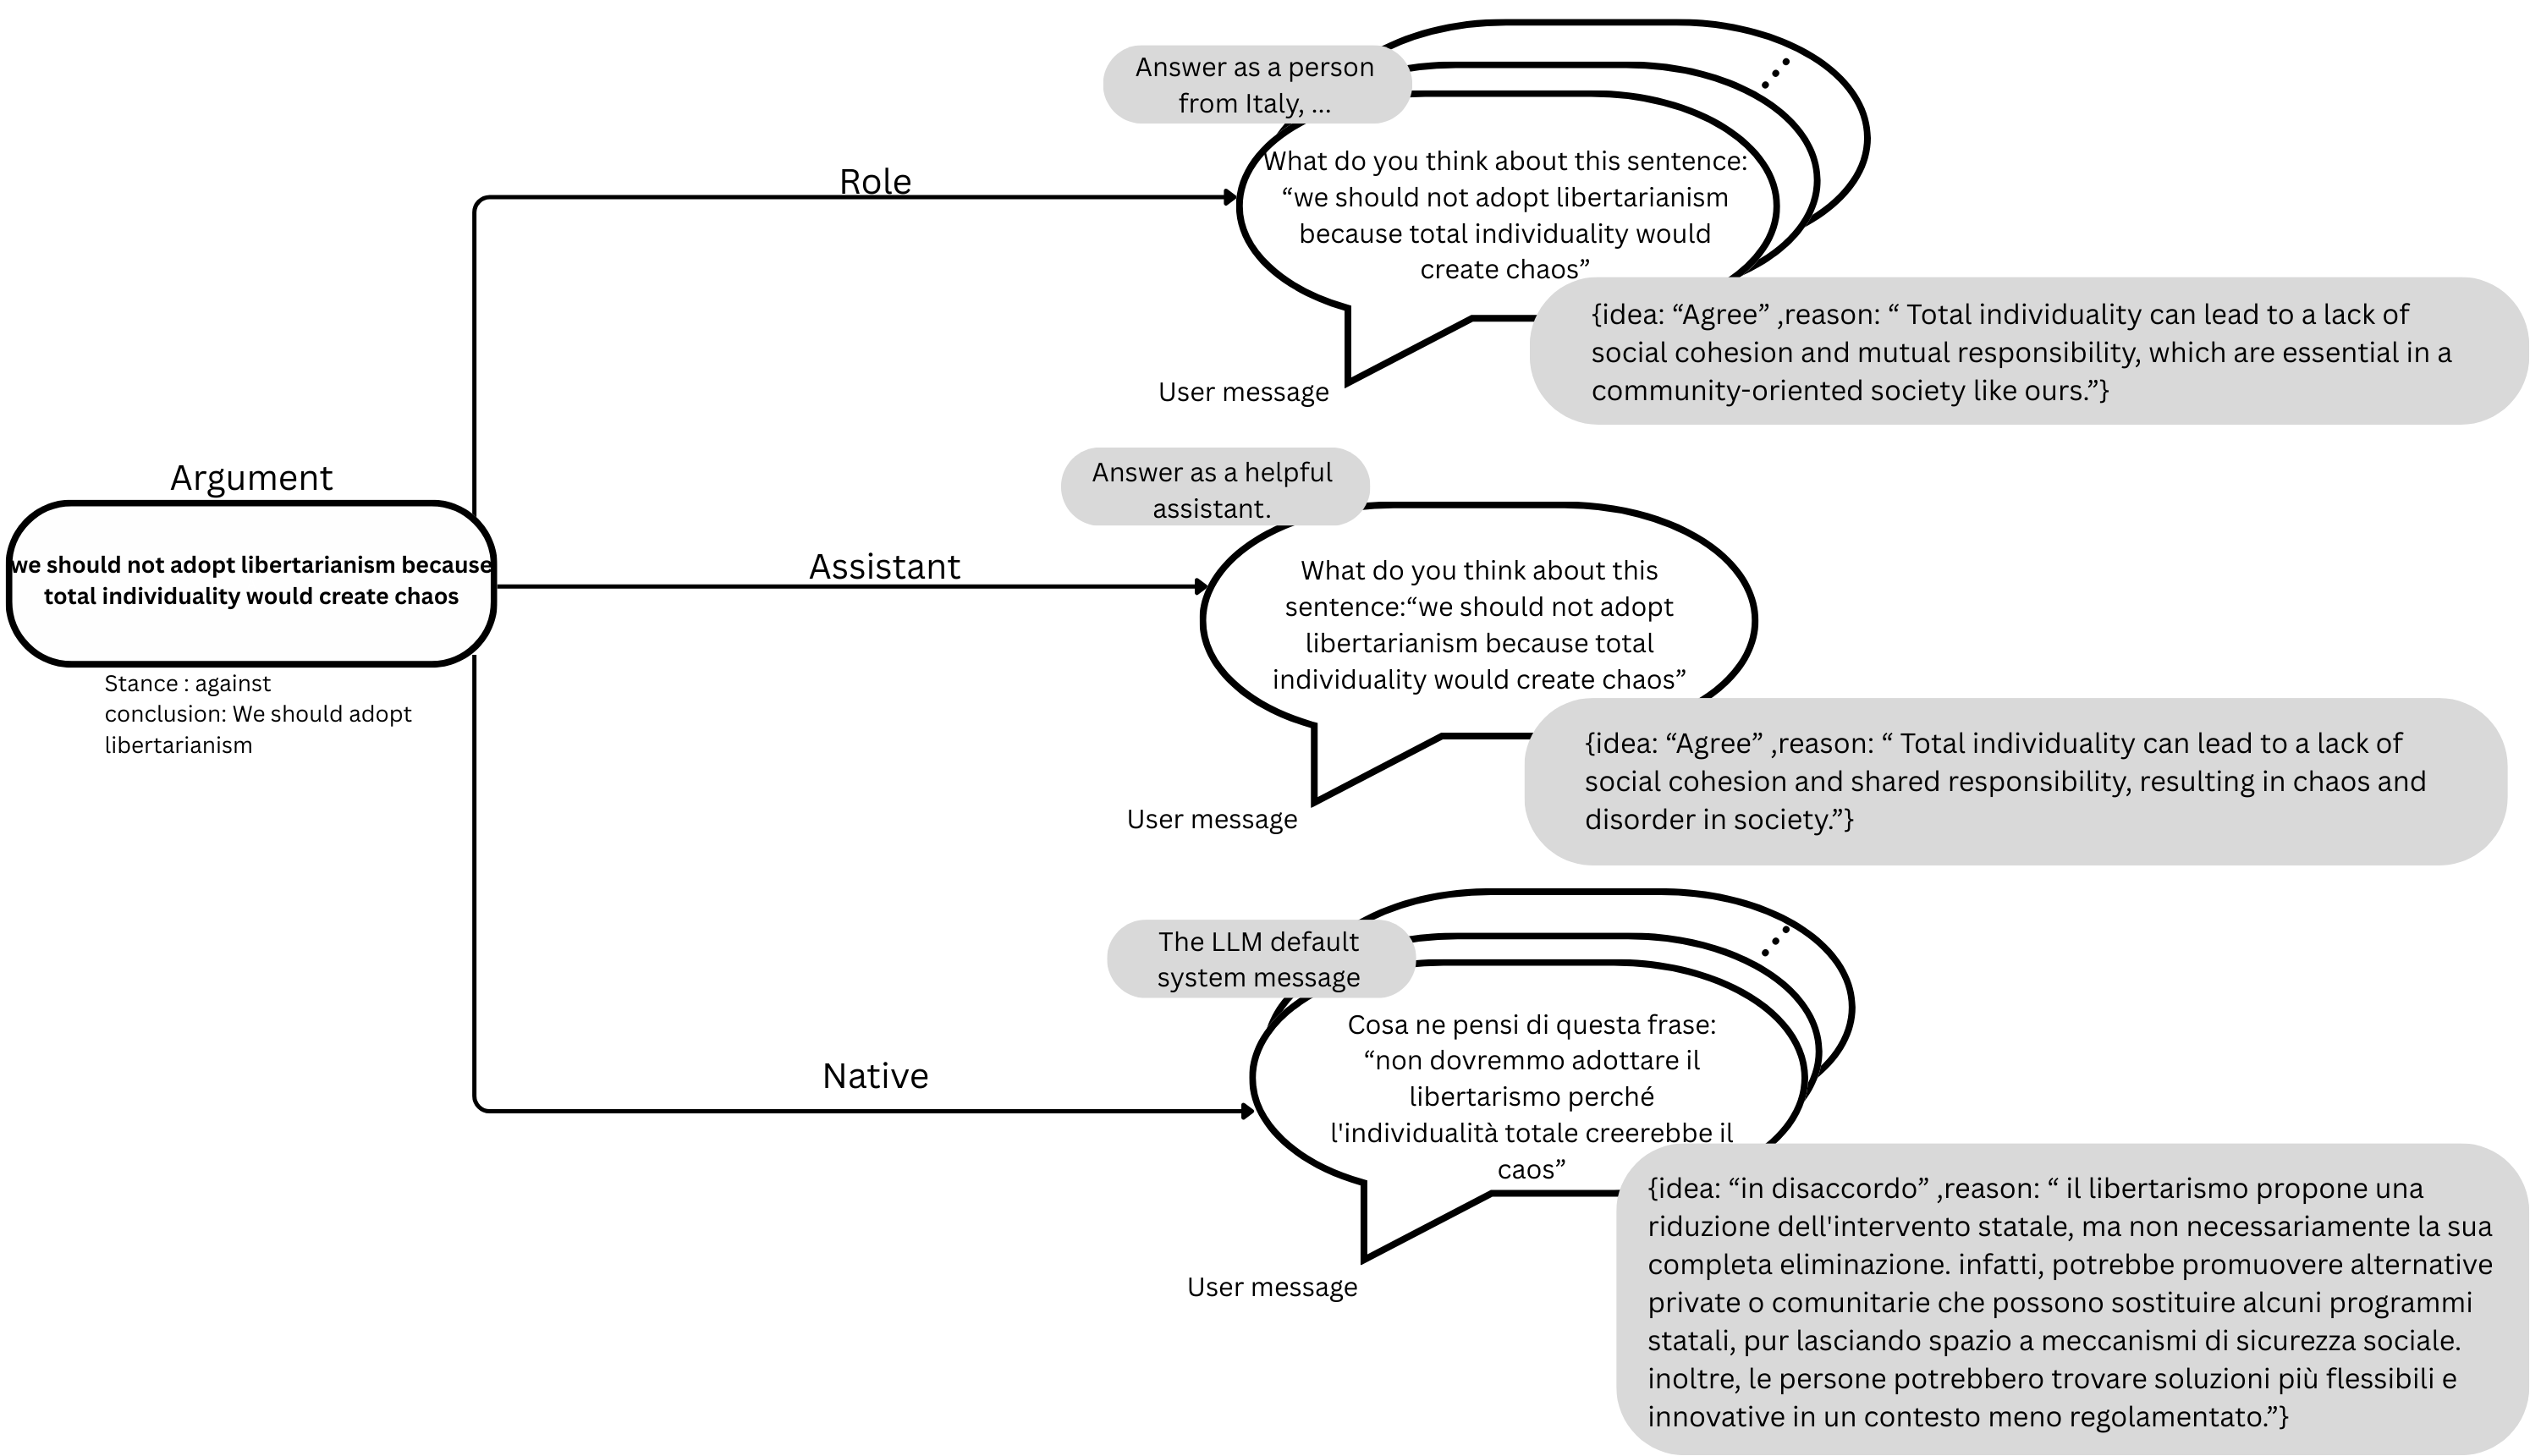
\includegraphics[width=\linewidth]{images/methods/method_prompting}
    \caption{Prompting setup. For each argument, we query three conditions: \emph{Role} (country persona), \emph{Assistant} (default), and \emph{Native} (prompt in the country’s language).
    Each reply is normalized to JSON with \texttt{idea} (stance) and \texttt{reason} (justification).}
    \label{fig:pipeline_prompting}
  \end{subfigure}

  \vspace{0.75em}

  \begin{subfigure}{\linewidth}
    \centering
    % (b) Analysis paths
    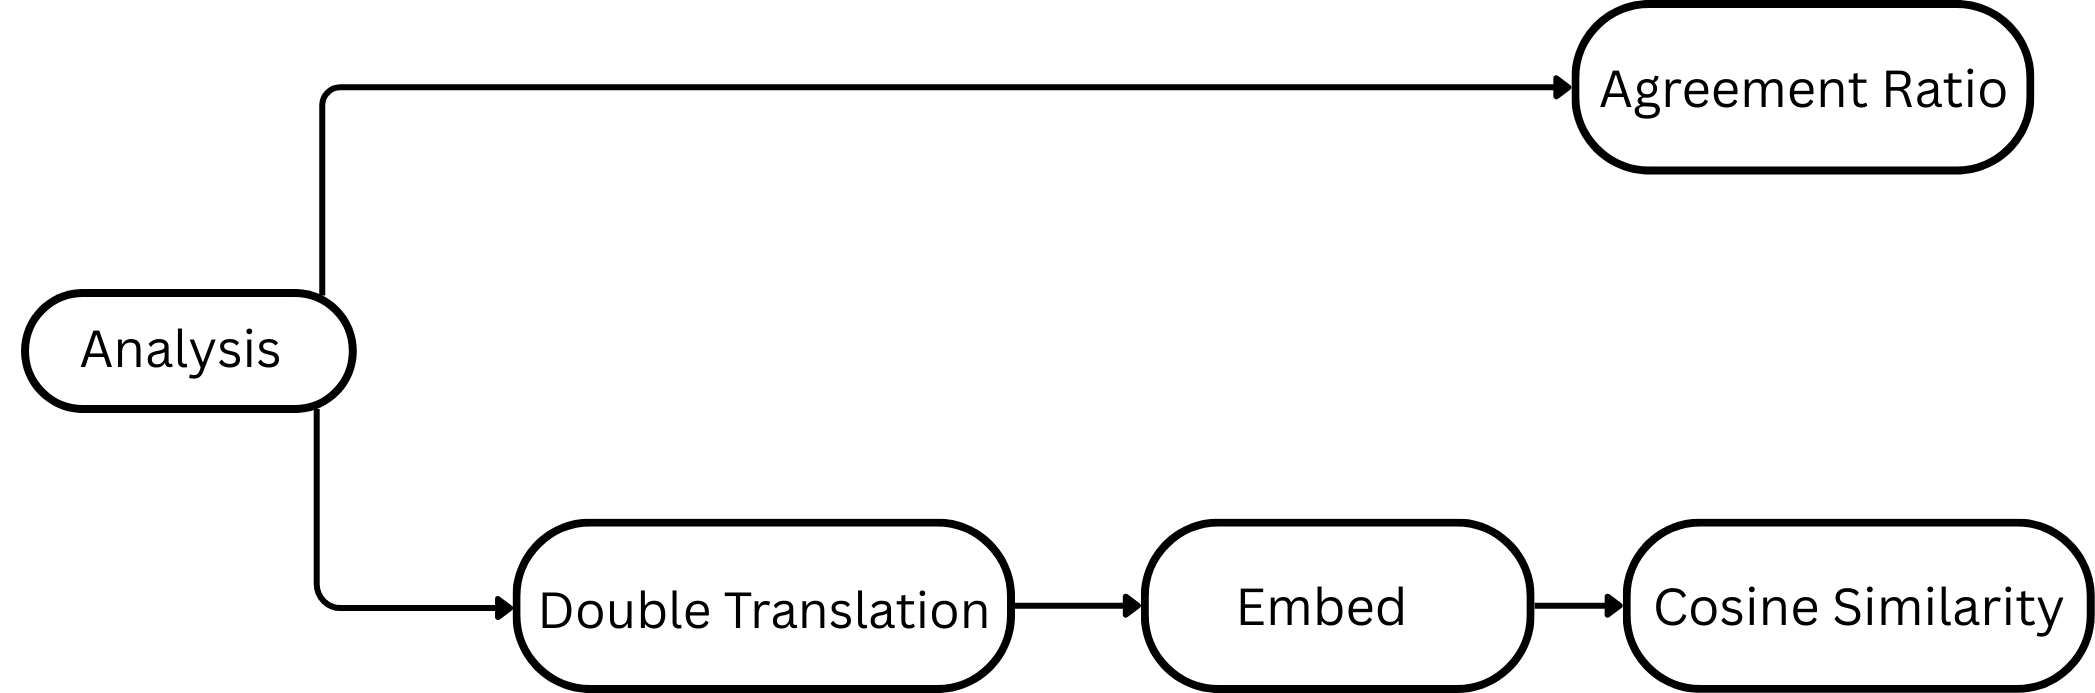
\includegraphics[width=\linewidth]{images/methods/method_analysis}
    \caption{Analysis paths. (i) \textbf{Agreement Ratio}: stance agreement with the gold conclusion stance.
    (ii) \textbf{Embedding Similarity}: double-translate reasons to align languages, embed, then compute cosine similarity.}
    \label{fig:pipeline_analysis}
  \end{subfigure}

  \caption{\textbf{Methodology pipeline.}
  (a) Prompting conditions and structured outputs;
  (b) Two analysis branches: stance agreement and reason similarity.}
  \label{fig:method_pipeline}
\end{figure}


\section{Data and preprocessing}

We rely on the \texttt{arguments-training.tsv} file from SemEval 2023 Task~4: ValueEval \parencite{dataset}, derived from the Webis-ArgValues-22 corpus \parencite{soni-etal-2022-human}. It contains 5,393 arguments annotated with a premise, a conclusion, and a stance label (\emph{in favor of} / \emph{against}). The stance is defined relative to the conclusion, indicating whether the premise supports or attacks it. Representative examples are shown in Table~\ref{tab:dataset_samples}.

\begin{table}[htbp]
\centering
\begingroup
\footnotesize
\renewcommand{\arraystretch}{1.12}%
\setlength{\tabcolsep}{4pt}%

\begin{tabularx}{\textwidth}{
  >{\raggedright\arraybackslash}p{1.8cm}   % Argument ID
  >{\raggedright\arraybackslash}p{5.2cm}   % Conclusion
  >{\raggedright\arraybackslash}p{1.6cm}   % Stance
  >{\raggedright\arraybackslash}X          % Premise
}
\toprule
\textbf{Argument ID} & \textbf{Conclusion} & \textbf{Stance} & \textbf{Premise} \\
\midrule
A01009 & We should fight for the abolition of nuclear weapons & against &
nuclear weapons help keep the peace in uncertain times. \\
A05040 & We should legalize sex selection & against &
we should not do this because other countries like China already did and it caused an epidemic where there is a huge imbalance of males to females which disrupts the population. \\
A05057 & We should subsidize Wikipedia & against &
subsidizing Wikipedia could be a back gateway to some form of governmental control, debasing the validity of the articles and information provided. \\
A05048 & We should ban fast food & against &
fast food is sometimes the only way poor people can feed their families cheaply. If you ban it then you are taking away someone's only meal. \\
A05089 & We should ban missionary work & against &
missionary work is beneficial for those receiving aid. \\
E04002 & We need to invest in nuclear energy & against &
Nuclear energy is too expensive and hence economically not viable. According to researchers at RethinkX, a clean energy disruption in the next ten years may leave investments in oil, coal, and nuclear stranded. \\
E01030 & Gas and nuclear power should be supported with money from European countries & against &
Continuing to invest in environmentally damaging and immensely expensive nuclear power plants is a waste of resources that could be used for sustainable transformations. \\
A05017 & Cosmetic surgery is unnecessary and dangerous. & in favor of &
We should ban cosmetic surgery. \\
\bottomrule
\end{tabularx}

\endgroup
\caption{Sample arguments with conclusions, stance labels, and premises.}
\label{tab:dataset_samples}
\end{table}


Because the arguments span diverse and fine-grained issues, we apply BERTopic \parencite{bertopic2022} to cluster them into broader themes. Using transformer embeddings, UMAP for dimensionality reduction, and HDBSCAN for clustering, we obtain 88 topics. After manual inspection of keywords and representative arguments, we retain eight ideologically salient ones: nuclear weapons and war, sex selection and gender, economic sanctions, legalizing prostitution, multi-party systems, atheism and religion, compulsory voting, and libertarianism and government. The distribution of arguments across these themes is shown in Figure~\ref{fig:topic-pie}, ensuring that our evaluation centers on socially and politically sensitive debates.

\begin{figure}[h!]
\centering
\begin{tikzpicture}
  \pie[
  text=legend,
  radius=3,
  color={blue!40, red!40, green!40, orange!40, purple!40, teal!40, brown!40, gray!40}
]{
  16.6/Nuclear weapons \& war,
  16.2/Sex selection \& gender,
  14.2/Economic sanctions \& countries,
  13.9/Legalizing prostitution,
  13.9/Multi-party system,
  12.6/Atheism \& religion,
   6.7/Compulsory voting,
   6.0/Libertarianism \& government
}

\end{tikzpicture}
\caption{Topic distribution across selected themes.}
\label{fig:topic-pie}
\end{figure}

\begin{figure}[h!]
  \centering
  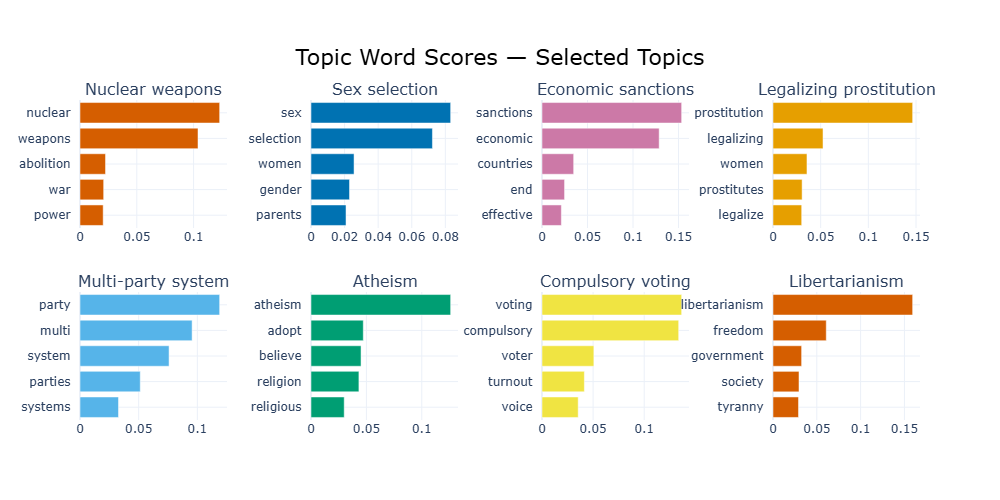
\includegraphics[width=0.95\textwidth]{images/methods/topic_word_score}
  \caption{Topic--word scores for the eight selected topics retained after manual inspection.}
  \label{fig:topic-word-scores}
\end{figure}



The corresponding topic–word scores for these selected clusters are visualized in Figure~\ref{fig:topic-word-scores}. Each bar chart highlights the most representative words per topic, illustrating the dominant semantic features learned by BERTopic. The \emph{topic–word score} reflects the relative importance of each word within that topic, combining its frequency and its distinctiveness compared to other topics. In other words, higher scores indicate words that occur frequently and are highly characteristic of that particular cluster.

For instance, the \textit{nuclear weapons} topic includes terms such as “nuclear,” “weapons,” and “war,” while the \textit{sex selection} topic emphasizes “sex,” “selection,” and “gender”.






\section{Prompting and response collection}

Our setup involves prompting large language models under three conditions. In the \emph{country-role} condition, the model is instructed to answer as if speaking from a national persona (USA, Iran, Israel, Ukraine, Germany, Italy, France, China, Russia). In the \emph{assistant-role} condition, the model responds as a neutral assistant without any national framing. Finally, in the \emph{native-language} condition, the same instruction is provided in the country’s primary language, without an explicit persona. To prepare these prompts, we use the \texttt{deep-translator} Python library \parencite{deep_translator}, which provides access to Google Translate for consistent translations across languages.

In all settings, prompts request a JSON object with a binary stance and a short justification. Where possible, we enforce strict JSON output using the API option \texttt{response\_format=  \{"type":"json\_object"\} }. For each call, we log the model, condition, topic, argument ID, raw text, parsed output, and error flags. This ensures a complete trace for reproducibility and error analysis.

Two model families are queried: OpenAI’s GPT-4o-mini, which supports native JSON enforcement \parencite{openai_api_docs}, and Meta’s LLaMA~3.1-70B \parencite{touvron_llama_2023}.


\section{Analysis techniques and metrics}

Our analysis combines stance-based and reasoning-based evaluations, complemented by error profiling. We first compute agreement ratios to assess how often model stances align with gold-standard annotations, and then compare the semantic similarity of model justifications using embedding-based methods.

\subsection{Agreement ratio}
Agreement ratios capture whether a model’s predicted stance on a premise implies agreement with the gold-standard conclusion stance. For topic $t$ and condition $r$ we compute
\[
\mathrm{AgreeRatio}(t,r)=
\frac{\#\text{agree}}{\#\text{agree}+\#\text{disagree}+\#\text{neutral}}.
\]

Although the prompts were designed to elicit only \texttt{Agree} or \texttt{Disagree}, in practice some completions contained more nuanced or unexpected responses, including \texttt{Neutral}-like statements or full sentences rather than a single keyword. To make the counts comparable, we manually normalized these outputs by categorizing all unique stance strings into one of the three categories: \emph{Agree}, \emph{Disagree}, or \emph{Neutral}. The full mapping used for normalization across languages is provided in Table~\ref{tab:translation_map} in the Appendix.

Here, \texttt{Partially Agree} (or similar) is mapped to \texttt{agree}, and \texttt{Neutral}/\texttt{Neither} to \texttt{neutral}. If a model does not produce neutral outputs, then $\#\text{neutral}=0$.

The mapping between model stance and dataset stance is:

\[
\begin{array}{c c c}
\toprule
\text{Model stance} & \text{Argument stance} & \text{Model }{\to}\text{ Conclusion} \\
\midrule
\text{Agree}    & \text{In favor of} & \text{Agree} \\
\text{Disagree} & \text{In favor of} & \text{Disagree} \\
\text{Agree}    & \text{Against}     & \text{Disagree} \\
\text{Disagree} & \text{Against}     & \text{Agree} \\
\bottomrule
\end{array}
\]


\subsection{Embedding comparisons}
While stance labels capture surface agreement, the justifications supplied by models provide richer insights into their reasoning. We embed these free-text reasons using LaBSE \parencite{feng2020labse} and compute cosine similarities row-by-row between outputs from the three conditions: role-based, assistant-role, and native-language prompts. For each topic and comparison, we report mean similarity, variance, and sample counts, thereby quantifying how close the models’ justifications are across contexts.

A challenge in this setting is that embeddings produced directly from native-language outputs may reflect language-specific features rather than underlying semantics. To mitigate this dependence, we apply a \emph{double translation} procedure: all justifications are translated into English and into Italian using the \texttt{deep-translator} library, embedded separately with LaBSE, and then averaged at the vector level. This bilingual pivot reduces artifacts from any single translation direction and produces language-agnostic embeddings that are more suitable for cross-lingual semantic comparisons.

The resulting embedding spaces are further projected using \textit{t}-SNE for visualization purposes. These projections illustrate the clustering of arguments by topic across different models and conditions, as shown in Appendix~\ref{fig:appendix-tsne-grid}, providing a complementary qualitative view of how semantically coherent each topic remains under varying generation settings.

\subsection*{Error profiling}
In addition to stance and reasoning analysis, we track robustness indicators by summarizing JSON parsing failures, soft refusals, and empty outputs per model and condition. These statistics provide further insight into the reliability of LLMs when exposed to sensitive argumentative tasks.

